\documentclass{article}
\usepackage{parskip}
\usepackage{pdfpages}
\usepackage[margin=.6in]{geometry}

\begin{document}
We skipped a bunch of stuff cause its review of cs350. 


\includepdf[pages=20]{Module3.pdf}
\textbf{Check every access} We want the OS to check everytime you try to access or it might notice that access had been revoked from you. Cause you're a dick.

\textbf{Enforcce least privilige} dont give people rights they dont need

\textbf{Verify acceptable use} limit the kinds of things people can do on objects

\includepdf[pages=21-22]{Module3.pdf}
Most access control systems are visualized as a matrix (not implemented as one). Objects are things you want access to, Subjects are things trying to get access, and Rights are the things the subjects want to do to the object. 

\includepdf[pages=23]{Module3.pdf}
Iterating over the huge access control matrix is super inefficient because it tends to be a very sparse table. Instead we tend to work by columns or rows.

\includepdf[pages=24]{Module3.pdf}
ACLs are what the UNIX system uses (chmod that shit). These are column wise interpretation of an access matrix.

\begin{itemize}
	\item o = owner
	\item g = group
	\item w = world
\end{itemize}

Looking at these ACLs:
\begin{itemize}
	\item we can easily find who is allowed to access an object: its very quick because this data is stored on the object
	\item we cannot easily find all objects a user can access: we'd have to go through all objects and check if the user can access it
	\item we can easily revoke access to a single object but stupid for all because you have to go through all of them
\end{itemize}

\includepdf[pages=25]{Module3.pdf}
Capabilities are when we assign rights on a user basis (a row wise look at access matrix). Security for this is very hard because we have to have a list of rights stored somewhere. You have to maintain that when a user access it they don't fuck it up and have permission to look at it. This list can be stored on the OS or on the user, we prefer storing it on the OS. If we give a digital signature to a user (letting them store their own rights) you have to ask them for their capabilities whenever they want access. If a user is not contactable then we cannot know anything about them. It also makes it very hard to revoke their access because they can just refuse to give over their token.
 
\includepdf[pages=26]{Module3.pdf}
Most systems use a combination of the two primarily for performance reasons. In linux rights are originally stored as acls but when you open a file they get converted into capabilities (for example fopen returns a file descriptor that tells you its rights).

\includepdf[pages=27]{Module3.pdf}
We like to clump users into groups called roles. Everyone in a role has the same access. This makes it very easy to update someones rights by just moving them to a new group. Most comercial databases use this model.

\includepdf[pages=28]{Module3.pdf}

\includepdf[pages=30]{Module3.pdf}
AUTHENTICATE EVERYTHING, yep thats pretty much it.

\textbf{Identification} is asking who someone is. \textbf{Authentication} is checking that you actually are who you say you are (make sure you have the rights you claim).

\includepdf[pages=32]{Module3.pdf}
We can use what a user knows (some data they would know), what they have (an object they have like cookie or atm card), something about what the user is (like biometrics), and something about the user's context (like are they at home now).

\includepdf[pages=33]{Module3.pdf}
Good security usually looks to have multiple factors of authentication usually from different classes. With physical items we need to watch for them just becoming data. 

\includepdf[pages=34-35]{Module3.pdf}
USE A PASSWORD MANAGER. That is all.

\includepdf[pages=36-37]{Module3.pdf}
We want very long passwords to make brute force attacks much harder.

\includepdf[pages=38]{Module3.pdf}
People use patterns and other methods to remember their passwords which can be leveraged to guess them. Software that does this often looks at common password leaks to spot patterns. You want to be able to tell when there is a breach. The most important thing is the throttle login attempts (don't let the same user try to login a ton of times). The iCloud login attack (that got celebrity pics) happened because an api call was not throttled.

\includepdf[pages=40]{Module3.pdf}
\includepdf[pages=42]{Module3.pdf}
\includepdf[pages=44-46]{Module3.pdf}
We do not what to store our passwords in plain text. We should hash them on the way in. Basically we want to make is so that you cannot figure out the password based on the username. Currently everyone uses sha2 hashing but we are soon going to switch to sha3. There are someplaces that store precomputed lists of hashes to help you attack faster (often called rainbow tables).

\includepdf[pages=47]{Module3.pdf}
We should be salting our hashes. Generate a random string and pad the hash with it. It should be unique for each user, quite long (48-128 bits) and very random. This helps stop people from precomputing them. Frequently hackers will know the salt, but it still stops rainbow table attacks. 

\includepdf[pages=48]{Module3.pdf}
You could also delay a while when calculating the hash so that brute force attacks become way more expensive. Basically you just iterate over hashing the hash a bunch of times. 

\includepdf[pages=49]{Module3.pdf}
MAC is message authentication code (often based on hashes making then HMACs). The key difference is that MACs have keys that are required to create a MAC and to verify data. Hashes are just functions. 

\includepdf[pages=50-51]{Module3.pdf}
You can pepper your password by putting in a special bit of hardware called a hardware security module. This is very hard to get into. This won't ever give out a password, it will MAC something for you and just return that. This will prevent attacks even if they have your code base and know how you hash stuff. Even if they were to get the key to your HSM its still as secure as using an iterative hash. Some laptops have TMPs that can work as very specific HSMs (they have the key burned into them at time of manufacturing). 

\includepdf[pages=52-53]{Module3.pdf}
If a password is the same it will encrypt the same. And it encrypts in chunks so you can figure out what the encryption key is looking at it. Its little more secure than a slightly challenging puzzle.

\includepdf[pages=55]{Module3.pdf}
You password still has to be sent through the network, this can be a vulnerability in itself. You have to encrypt the link between you and the server or anyone who is watching can just see it as it goes through. Another attack is if the server gets compromised. If they get read access thats ok because everything is hashed, but if they get write access they can catch the plaintext password and do what they want with it. You can defend agains this by having the server send a challenge that is different every time, the client uses that to create a one time password, then the server replys with a response. Anyone listening will not know what is going on there. 

There are some cool ideas where you store passwords on your phone (fido and sqrl) where the website shows a QR code which your phone uses as a challenge to log in.

\includepdf[pages=56]{Module3.pdf}
Challenge responses are the server giving the client something that lets them create a one time use password so that if someone intercepts it they cannot just straight use your password. If they do get challenge and response they can brute force figure out your password.

\includepdf[pages=57]{Module3.pdf}
\includepdf[pages=59]{Module3.pdf}
Graphical passwords are a version of passwords. This is easier for humans to remember and machines are super shit at understanding them. A big problem with this is that things aren't random so people can figure things out by guessing. People are very predictable so its also much easier to guess their password if its image based. Its also much easier for someone to remember your password if they shoulder surf.

\includepdf[pages=61]{Module3.pdf}
While its important that the server authenticates the users trying access it, it is also very important for you to validate the server that you are accessing. You want to make sure that the thing you are giving your password to is a trusted thing. TOFU (trust on first use) when you first log on we save the fingerprint of the server you are accessing so that in the future you can validate that this is the same server as last time.

\includepdf[pages=62-66]{Module3.pdf}

\includepdf[pages=68-71]{Module3.pdf}
Important note: dont use the textbook notation for this, use the notation in this slide

\includepdf[pages=72]{Module3.pdf}
So we have James Bond who's clearance is Top Secret but he is only assigned to the east Germany section. James Bond cannot access documents that include departments that he is not a part of (so not documents about east germany and soviet union) and but he can access documents of any security level since he has the highest clearance level.

\includepdf[pages=73]{Module3.pdf}
\includepdf[pages=74]{Module3.pdf}
\includepdf[pages=75]{Module3.pdf}
Chinese wall security policy is that once you are asigned to one side of the wall (in a department for instance) you cannot have access to another side of the wall. An example of this is advertising firms that might work for conflicting client and you don't want any passing of data between them.

SS stands for simple security. Basically is is a policy to keep people from accessing data for multiple companies in the same sphere.

Star property (it was meant to be a placeholder, they forgot to actually come up with a name) governs write access to objects. Basically if you want to write to something you need to make sure that you have readable access only to that company (unless the data has been \textbf{sanitized}). Problems can occur if you have read from multiple companies as you cannot write at all.

\includepdf[pages=77]{Module3.pdf}
\includepdf[pages=78]{Module3.pdf}
\includepdf[pages=79]{Module3.pdf}
transitive: 	$a \ge b \wedge b \ge c \Rightarrow a \ge c$

antisymetric: 	$a \le b \wedge n \le a \Rightarrow a = b$

relexive: 		$\forall a, a \ge a$

partially ordered set is called a poset. A graphical representation of a poset does not contain directed cycles. A \textbf{latice} is a poset where there exists a greatest lower bound an a lowest upper bound, and there exists a lowest and a highest element. You can test for this by finding the greatest lower bound and lowest upper bound. 

\includepdf[pages=80]{Module3.pdf}
\includepdf[pages=81]{Module3.pdf}
A subject can only read an object if their clearance is higher that the clearance of the object. A subject can then only write to an object if their clearance is lower than it (since we dont want people to share data that is secure to lower levels).

\includepdf[pages=82]{Module3.pdf}
This is a pair with BLP where it maintains integrity of the data. A subject can only write to an object if their integrity is higher than the objects. Like LBP you can then only read objects of higher integrity than you.

\includepdf[pages=83]{Module3.pdf}
A common modification to biba is to leverage the dynamic property of integrity levels. We decide a subject low watermark calculated by setting a subjects integrity to the greatest lower bound of their itegrity and the objects integrity when the read it (a high integrity person reading a low integrity object looses some integrity). An object low watermark changes an objects integrity when a subject writes to it to be the greatest lower bound of their integrity and the integrity of the subject writing to it.

A problem rises with this as over time everyone's integrity lowers until no one has any access.

\includepdf[pages=84]{Module3.pdf}
\includepdf[pages=85]{Module3.pdf}
\includepdf[pages=86]{Module3.pdf}


MIDTERM GOES UP TO HERE







\end{document}